% Copyright (c)  2019  FSC.
% Permission is granted to copy, distribute and/or modify this document
% under the terms of the GNU Free Documentation License, Version 1.3
% or any later version published by the Free Software Foundation;
% with no Invariant Sections, no Front-Cover Texts, and no Back-Cover Texts.
% A copy of the license is included in the section entitled "GNU
% Free Documentation License".

\chapter{Piano di qualità}\label{chap:piano-qualita}

\section{Analisi dei rischi}\label{sec:analisi-rischi}
L'analisi dei rischi si è incentrata sulla stesura di un documento di 
\textit{Privacy Policy} che riguarda il trattamento dei dati inseriti 
dall'utente, la loro conservazione e l'impegno del gruppo di offrire gli 
standard di sicurezza più elevati. 

Il suddetto documento è consultabile tramite il seguente link alla 
\href{https://f-s-c.github.io/emotionally_policy/privacy_policy.html}{Privacy 
Policy} \url{https://f-s-c.github.io/emotionally_policy/privacy_policy.html}.

\section{Piano del progetto}\label{sec:piano-progetto}
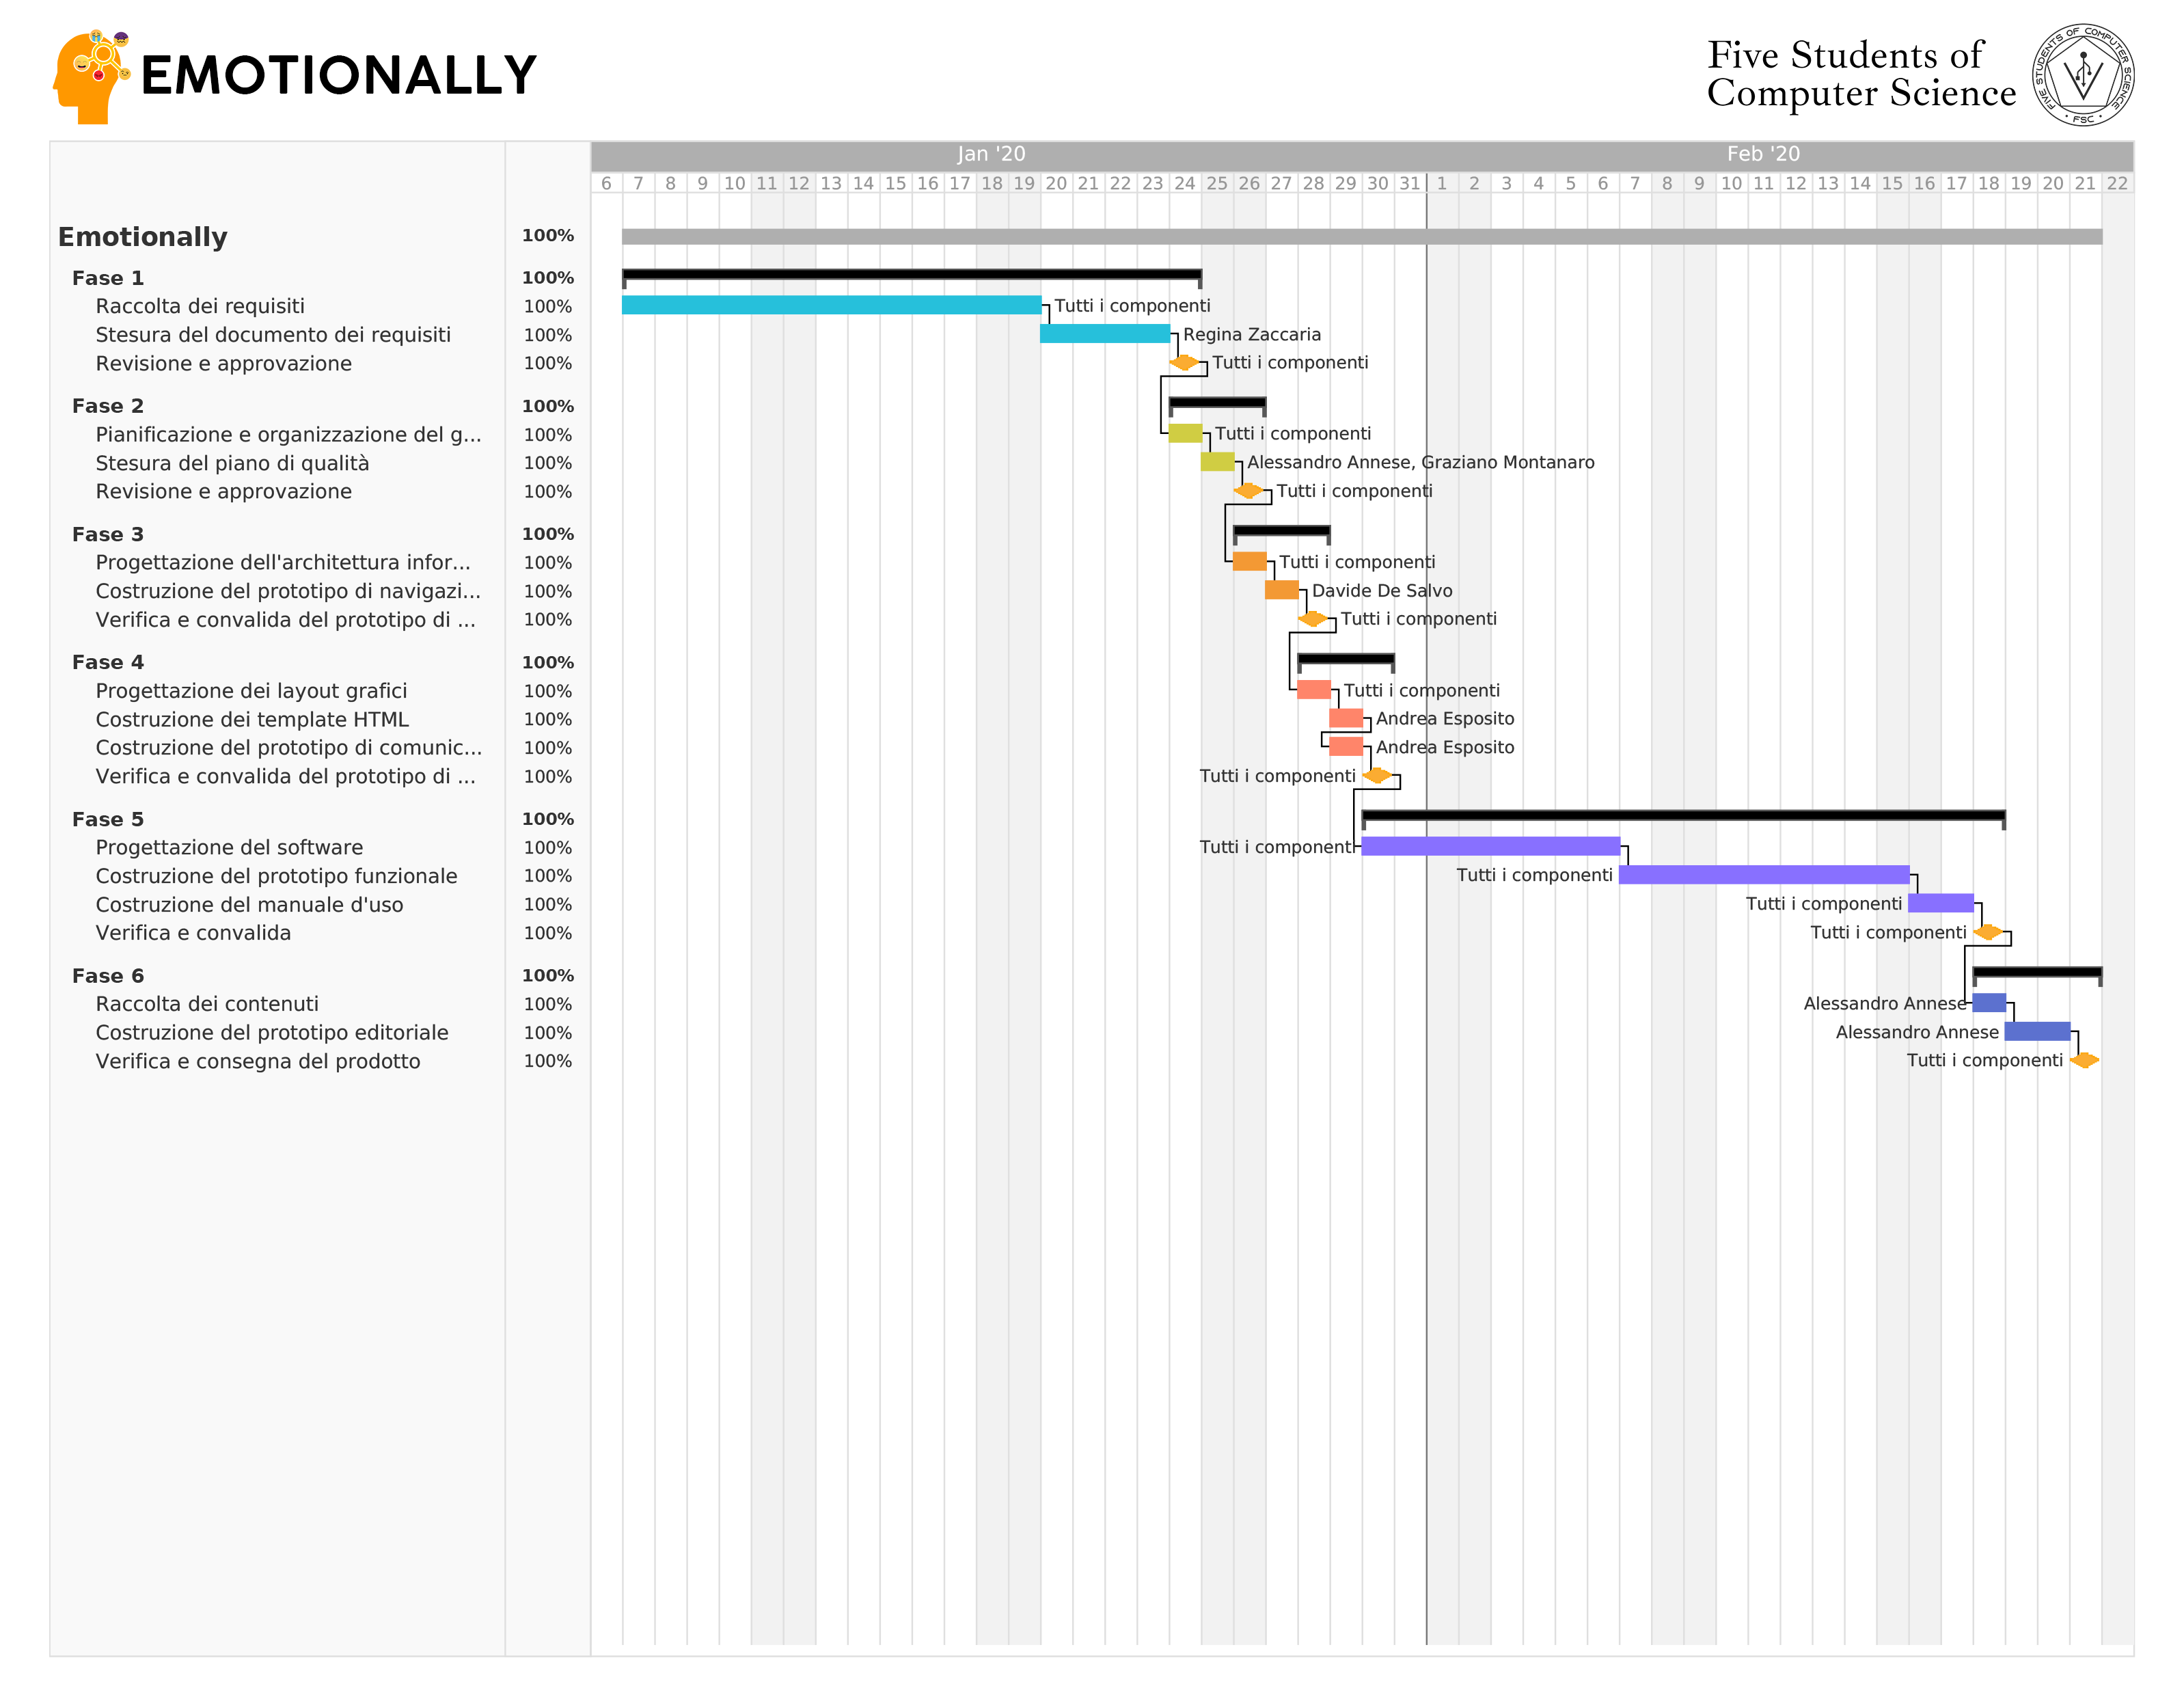
\includegraphics[height=11.5cm, frame]{images/gantt.png}

\section{Organizzazione del gruppo}\label{sec:organizzazione-gruppo}
Il gruppo, dopo essersi riunito in un brainsorming iniziale, ha deciso di 
dividersi in maniera modulare assegnando ad ogni componente un compito 
specifico.\\
In ogni fase, tutti i componenti del gruppo si riuniscono per una 
pianificazione iniziale e, alla fine di essa, si occupano  di verificare e 
convalidare il lavoro svolto.\\
Di seguito viene riportata la suddivisione dei compiti:

\begin{itemize}
	\item \textbf{Fase 1}\\
	In questa fase è prevista, oltre alla raccolta dei requisiti effettuata da 
	tutto il team, la stesura del documento dei requisiti. Quest'ultima è stata 
	assegnata a \textit{Regina Zaccaria}. Alla stesura hanno partecipato 
	\textit{Davide De Salvo} che ha realizzato le gabbie di massima del sito, 
	\textit{Alessandro Annese} che si è occupato della progettazione 
	concettuale del database e \textit{Andrea Esposito} che ha sistemato alcuni 
	errori grafici dei diagrammi, tabelle e gabbie logiche. 
	
	Il termine della fase è stato fissato per il 24/01/2020.
	\item \textbf{Fase 2}\\
	La stesura del piano di qualità è stata assegnata a \textit{Alessandro 
	Annese} e \textit{Graziano Montanaro}.
	
	Il termine della fase è stato fissato per il 26/01/2020.
	\item \textbf{Fase 3}\\
	La creazione del prototipo di navigazione è stata effettuata da 
	\textit{Davide De Salvo}. Il prototipo è stato realizzato con \texttt{Adobe 
	XD}.
	
	Il termine della fase è stato fissato per il 28/01/2020.
	\item \textbf{Fase 4}\\
	La costruzione dei template di base in \texttt{HTML} e del prototipo di 
	comunicazione è stata affidata a \textit{Andrea Esposito}.
	
	Il termine della fase è stato fissato per il 30/01/2020.
	\item \textbf{Fase 5}\\
	In questa fase si è progettato il software costruendo il prototipo 
	funzionale e, successivamente, si è redatto il manuale d'uso. Tutti i 
	membri del team si sono occupati di completare l'intera fase.
	
	Il termine della fase è stato fissato per il 18/02/2020.
	\item \textbf{Fase 6}\\
	La raccolta dei contenuti e successiva creazione del prototipo editoriale 
	sono stati affidati a \textit{Alessandro Annese}. Successivamente al 
	completamento della fase si è occupato anche di effettuare la consegna del 
	prototipo con la relativa documentazione al committente.
	
	Il termine della fase e relativa consegna del prodotto è fissato per il 
	21/02/2020.
\end{itemize}

